\subsubsection{Tour improvement}

An improvement heuristic is an algorithms that works over a valid and complete solution, in order to improve it. The most common improvement heuristics are the 2-opt and 3-opt local search procedures \cite{lkh_original}, and the Lin-Kernighan algorithm (LK) . The latter is a particular implementation of the former two local searches methods, in which a $k$-opt local search is employed, but the value of $k$ varies during the algorithm execution. The LK algorithm is very efficient and capable of presenting high quality solutions for the symmetric TSP.

The 2-opt is a simple iterative local search procedure, in which two arcs of the solution are removed, and a new solution is constructed by reconnecting the nodes in a different way. Given that only 2 arcs are exchanged, there is only one way of creating a different cycle. Note that by performing a 2-opt exchange, the path between the two exchanged arcs get reversed. If the graph is symmetric, the objective function difference can be calculated by analyzing two arcs only. However, if the graph is asymmetric, it is necessary to recalculate the cost of the new path, as to evaluate the objective function difference. This makes the 2-opt procedure particularly efficient for symmetric problems, but lacks performance for the asymmetric, and as a consequence, the time-dependent variations of the TSP. 

\todo{Acertar isto.}

%The 2-opt is one of the most simple local search procedures. The goal of this procedure is to find route crossovers, and fold them. This process is illustrated in figure $\ref{fig:two_opt_move}$. When this occurs, the overall cost of the newly constructed tour will decrease. The 2-opt search works in a recursive way. It tries to improve the original tour, by removing two edges from the original cycle, and reconnecting the two paths created. In a 2-opt search, there is only one way of connecting the nodes in a way that will result in a different and valid tour. If the new tour has a lower cost, the cycle restarts, using the new tour as the improvement object. Otherwise, two other edges are selected, and the cycle continues with the original solution. This iterative method continues until no further improvement is reached over a complete iteration cycle. In this case, the tour is known to be 2-opt.

\begin{figure}[htpb]
  \centering
  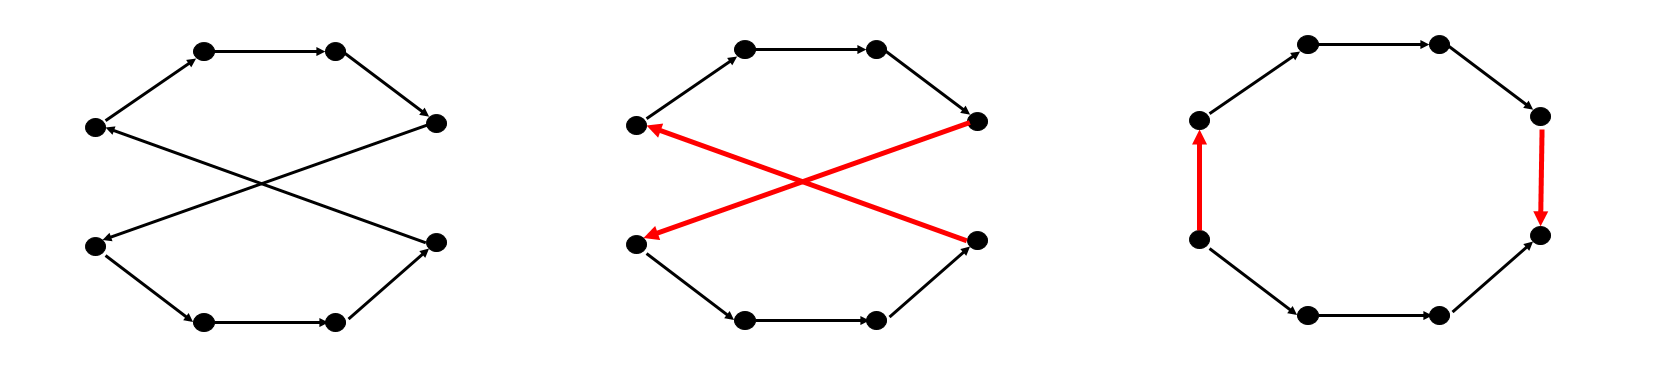
\includegraphics[width=.7\textwidth]{./Figures/tsp/2-opt-explained}
  \caption{The 2-opt local search reconnects two edges, hoping to
  fold possible crossovers, decreasing the overall tour cost. In the left image,
  a crossover is identified. In the middle image, the edges belonging to this crossover
  are removed, and in the figure to the right, they are reconnected, forming a new valid tour.}
  \label{fig:two_opt_move}
\end{figure}

The 3-opt search is very similar to the 2-opt, but instead of selecting two edges and reconnecting the path, the 3-opt selects 3 edges. In this case, there are multiple ways of forming a new valid tour. A 3-opt move can also be seen as two or three 2-opt moves combined in the formation of a new tour. The iterative cycle of the 3-opt search works in the same way as the 2-opt.

More generally, the $k$-opt local search is a method for rearranging a tour, by taking $k$ edges and reconnecting the paths in order to form a new valid tour. Any tour that is known to be $k-opt$ is also $(k-1)$-opt. Some particular problems, as \textit{the crossing bridges}, illustrated in figure $\ref{fig:crossing_bridges}$, can only be solved with a 4-opt or higher method.

\begin{figure}[htbp]
  \centering
  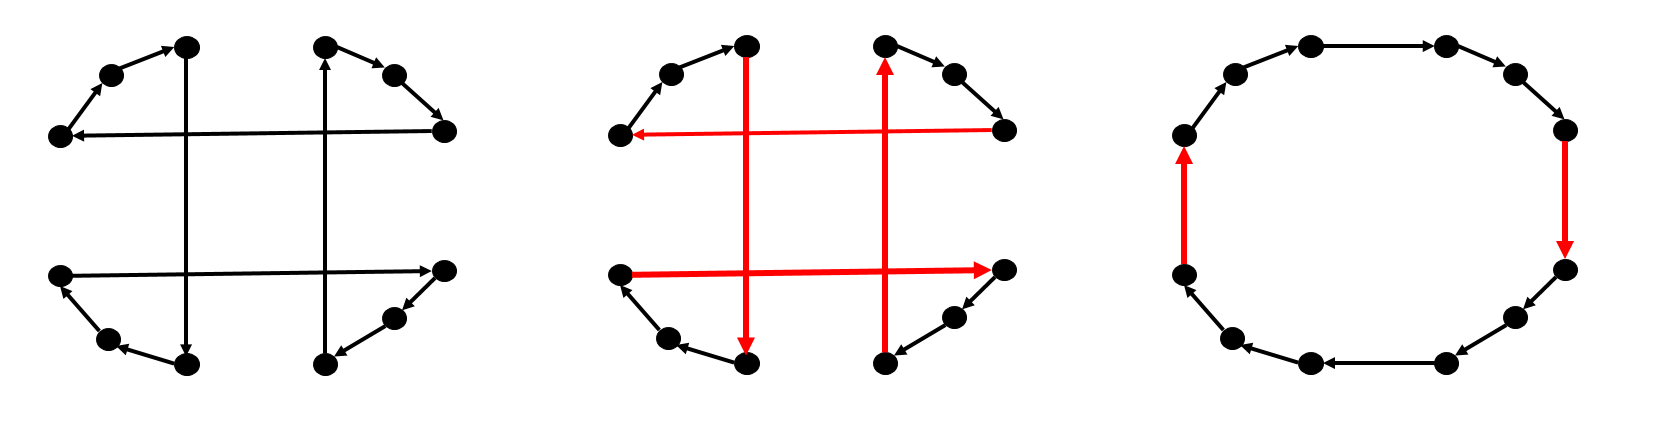
\includegraphics[width=.7\textwidth]{./Figures/tsp/crossing_bridges}
  \caption{The crossing bridges can only be solved by reordering 4 edges.
  The resolution of this problem with local search is only possible
  with 4-opt or higher.}
  \label{fig:crossing_bridges}
\end{figure}


In its turn, the Lin-Kernighan heuristic \cite{lkh_original} is an algorithm for the resolution of  the symmetric TSP, and it was the state of the art for over 15 years. LK is known for producing high quality solutions, some of them optimal, and for having a time complexity of approximately $\mathcal{O}^{n^{2.2}}$ \cite{heuristics_tsp}. This heuristic is restricted to the  the symmetric TSP, and using it for asymmetric instances requires a graph transformation, which transforms the asymmetric instance with $n$ nodes, into an equivalent symmetric one with $2n-1$ nodes (\cite{atsp_to_tsp_1}, \cite{atsp_to_tsp_2}). Thus, for the same number of nodes, solving an asymmetric TSP with the LK heuristic is usually 4 times harder than solving the symmetric case.

To understand the Lin-Kernighan heuristic, it is necessary to think about the TSP in a slightly different manner. Consider the following way of defining a combinatorial optimization problem: "find, from a set $S$, a subset $T$ that satisfies some criterion $C$ and minimizes an objective function $f$." In the TSP, the objective is to find, from the set of all edges ($S$) of a complete graph, the subset ($T$) which forms a valid tour ($C$) and minimizes the objective function ($f$). 

Any non-optimal but feasible solution $T$ is non-optimal because $k$ elements $\{x_1, ..., x_k\}$ in T are \textit{out of place}. To improve this solution, and make it optimal, one would have to substitute the set of $k$ elements $x_1, ..., x_k$ with the elements $y_1, ..., y_k$ of $S \backslash T$. Because there is no knowledge about how many elements are misplaced, Lin and Kernighan consider that setting the value of $k$ a priori would seem artificial. Thus, they propose an iterative procedure in which the algorithm dynamically estimates the best value for $k$. In order to do this, the LK first estimates the most out of place elements, $x_1$ and $y_1$. With these values set aside, it tries to repeat this process for $x_2$ and $y_2$, and so on. This inner loop stops when no improvement seams plausible and, at this point, it replaces the current solution $T$ with the new solution generated from replacing the now selected elements, and restarts the whole process. 



